\subsection{Transcription-regulator enrichment (UniProt): present in conserved targets, absent in CNN non-conserved targets}
Conserved miRNA targets are known to be enriched for transcription regulators. We test whether CNN non-conserved targets share this property using UniProtKB release 2026\_03 (reviewed human entries with keyword KW-0805, 2,374 of 20,190; script and results: \texttt{uniprot\_tf\_enrichment}; hermetic tests). The statistic is the fraction of a 200-gene set carrying KW-0805; site-count and expression-matched controls were fixed in advance.
Gates passed. The positive control recovers the classic result: TargetScan conserved top-200 sets are richer in transcription regulators than random UTR genes for 13/13 miRNAs ($p=1.2\times10^{-4}$), and KW-0805 prevalence is 11.8\%. CNN top-200 sets show no enrichment: versus uniform random 6/7 ($p=0.709$), versus site count 4/9 ($p=0.954$), versus expression-matched 7/6 ($p=0.500$); all three are falsified (Figure~\ref{fig:uniprot}).
Together with the GTEx avoidance result this is the second functional signature that conserved targets carry and CNN non-conserved candidates lack. The same caveat applies: conservation and scorer are confounded, and the universes differ between arms.
\begin{figure}[h]\centering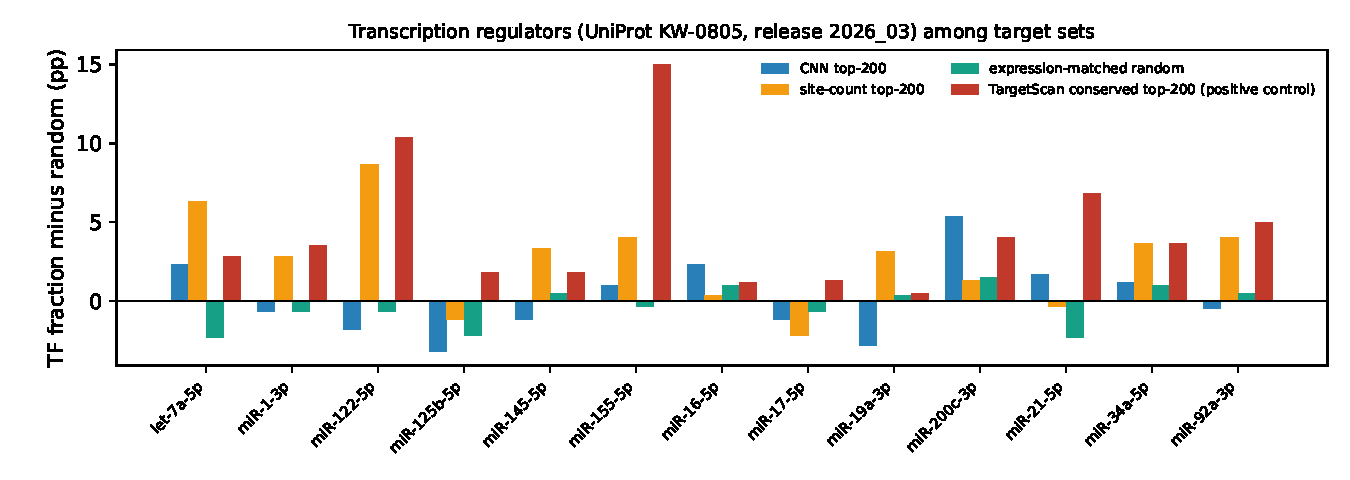
\includegraphics[width=0.95\linewidth]{figs/fig_uniprot.pdf}
\caption{Transcription-regulator fraction of each 200-gene set minus its random baseline (percentage points). Red: TargetScan conserved targets against random UTR genes (positive control).}\label{fig:uniprot}\end{figure}
